\documentclass{elektr}

% Anonymous initial-submission manuscript prepared with the official
% Turkish Journal of Electrical Engineering and Computer Sciences class.
\usepackage{hyperref}
\hypersetup{colorlinks=true,urlcolor=black,citecolor=blue}
\usepackage{amsfonts,amssymb,amsmath,amsgen,amsopn,amsbsy,theorem,graphicx}
\usepackage[utf8]{inputenc}
\usepackage[english]{babel}
\usepackage{booktabs}
\usepackage{array}
\usepackage{multirow}
\usepackage{url}
\usepackage{microtype}
\usepackage{comment}
\usepackage{enumitem}
\usepackage{tikz}
\usetikzlibrary{arrows.meta,calc,fit,positioning,backgrounds}
\usepackage[pagewise]{lineno}
\linenumbers

% Compact, journal-compatible algorithm blocks following the supplied
% manuscript style: horizontal rules, Require/Ensure lines, and numbered steps.
\newcounter{algorithmblock}
\newenvironment{algorithmblock}{%
  \par\medskip\noindent\begin{minipage}{0.96\linewidth}\small
  \setlength{\parindent}{0pt}%
  \hrule height 0.45pt%
  \vspace{4pt}%
}{%
  \vspace{4pt}%
  \hrule height 0.45pt%
  \end{minipage}\par\medskip
}
\newcommand{\algtitle}[1]{%
  \refstepcounter{algorithmblock}\textbf{Algorithm \thealgorithmblock}\quad #1\par\smallskip
}
\newcommand{\algrequire}[1]{\textbf{Require:} #1\par}
\newcommand{\algensure}[1]{\textbf{Ensure:} #1\par\smallskip}
\newenvironment{algsteps}{%
  \begin{enumerate}[label=\arabic*:,leftmargin=2.15em,labelsep=0.55em,
                    itemsep=1pt,topsep=1pt,parsep=0pt]
}{%
  \end{enumerate}
}
\newcommand{\algstep}[1]{\textbf{#1}\par\smallskip}
\newcommand{\algline}[1]{\hspace*{1.5em}#1\par\smallskip}

\yil{}\vol{}\fpage{}\lpage{}\doi{}

\title{Reinforcement learning-based adaptive filter selection for PPG-derived heart rate estimation}

% Identity-bearing information is supplied only in titlepage.tex.
\author[Anonymous]{}

\def\E{\ifmmode{\mathbb E}\else{$\mathbb E$}\fi} %natural numbers
\def\N{\ifmmode{\mathbb N}\else{$\mathbb N$}\fi} %natural numbers
\def\R{\ifmmode{\mathbb R}\else{$\mathbb R$}\fi} %real numbers
\def\Q{\ifmmode{\mathbb Q}\else{$\mathbb Q$}\fi} %rational numbers
\def\C{\ifmmode{\mathbb C}\else{$\mathbb C$}\fi} %complex numbers
\def\H{\ifmmode{\mathbb H}\else{$\mathbb H$}\fi} %complex numbers
\def\Z{\ifmmode{\mathbb Z}\else{$\mathbb Z$}\fi} %integers
\def\P{\ifmmode{\mathbb P}\else{$\mathbb P$}\fi} %real numbers
\def\T{\ifmmode{\mathbb T}\else{$\mathbb T$}\fi} %real numbers
\def\SS{\ifmmode{\mathbb S}\else{$\mathbb S$}\fi} %real numbers
\def\DD{\ifmmode{\mathbb D}\else{$\mathbb D$}\fi} %real numbers

\renewcommand{\a}{\alpha}
\renewcommand{\b}{\beta}
\renewcommand{\d}{\delta}
\newcommand{\D}{\Delta}
\newcommand{\e}{\epsilon}
\newcommand{\var}{\varepsilon}
\newcommand{\g}{\gamma}
\newcommand{\la}{\lambda}
\newcommand{\La}{\Lambda}
\newcommand{\lan}{\langle}
\newcommand{\ran}{\rangle}
\newcommand{\n}{\nabla}
\newcommand{\va}{\varphi}
\newcommand{\s}{\sigma}
\newcommand{\Sig}{\Sigma}
\renewcommand{\t}{\tau}
\renewcommand{\th}{\theta}
\newcommand{\Om}{\Omega}
\newcommand{\om}{\omega}
\newcommand{\pa}{\partial}
\newcommand{\up}{\upsilon}
\newcommand{\vp}{\varphi}
\newcommand{\z}{\zeta}





\newcommand{\bse}{\begin{subequations}}
\newcommand{\ese}{\end{subequations}}
\newcommand{\ben}{\begin{enumerate}}
\newcommand{\een}{\end{enumerate}}
\newcommand{\bens}{\begin{enumerate*}}
\newcommand{\eens}{\end{enumerate*}}
\newcommand{\be}{\begin{equation}}
\newcommand{\ee}{\end{equation}}
\newcommand{\bea}{\begin{eqnarray}}
\newcommand{\eea}{\end{eqnarray}}
\newcommand{\baa}{\begin{eqnarray*}}
\newcommand{\eaa}{\end{eqnarray*}}
\newcommand{\bc}{\begin{center}}
\newcommand{\ec}{\end{center}}
\newcommand{\ol}{\overline}
\newcommand{\ul}{\underline}
\newcommand{\ov}{\overbrace}
\newcommand{\uv}{\underbrace}
\newcommand{\Ra}{\Rightarrow}
\newcommand{\ra}{\rightarrow}
\newcommand{\ds}{\displaystyle}
\newcommand{\vs}{\vspace}


\newcommand{\IR}{\mbox{I \hspace{-0.2cm}R}}
\newcommand{\IN}{\mbox{I \hspace{-0.2cm}N}}



%% \theoremstyle{plain} %% This is the default

\newtheorem{theorem}{Theorem}%[section]

\theoremstyle{corollary}
\newtheorem{corollary}{Corollary}

\theoremstyle{lemma}
\newtheorem{lemma}{Lemma}

\theoremstyle{proposition}
\newtheorem{proposition}{Proposition}

\theoremstyle{axiom}
\newtheorem{axiom}{Axiom}

\theoremstyle{conjecture}
\newtheorem{conjecture}{Conjecture}

\theoremstyle{example}
\newtheorem{example}{Example}

\theoremstyle{definition}
\newtheorem{definition}{Definition}%[section]

\theoremstyle{remark}
\newtheorem{remark}{Remark}%[section]
\newtheorem{notation}{Notation}


\newtheorem{question}{Question}%[section]
\newtheorem{construction}{Construction}

\newtheorem{athm}{Theorem}
\renewcommand{\theathm}{\Alph{athm}}




\setcounter{page}{1}

\begin{document}
\maketitle

\begin{abstract}
Photoplethysmography (PPG) heart-rate estimation is affected by waveform distortion, transient peak ambiguity, and subject-dependent morphology. We formulate filter selection as a sequential decision problem and test whether a transparent tabular reinforcement-learning (RL) controller can select a preprocessing action for each consecutive PPG window. The state contains a label-free signal-quality index, normalized entropy, peak quality, the previous heart-rate estimate, and the previous action. Six actions encode the raw signal, two moving averages, a Savitzky--Golay filter, and two parameterized Butterworth band-pass filters. All 53 recordings in the BIDMC PPG and Respiration Dataset were retained. Eight-second windows with a four-second stride produced 119-window subject episodes, and five-fold subject-grouped cross-validation prevented windows from a subject appearing in both training and test sets. Every-visit Monte-Carlo, off-policy Q-learning, on-policy SARSA, contextual-bandit, fixed-filter, and supervised action-classification baselines were evaluated with MAE, RMSE, Pearson correlation, Bland--Altman agreement, paired tests with Holm correction, state ablation, and exploration sensitivity. Across 53 held-out subjects, Q-learning achieved MAE $3.840\pm8.965$ BPM and RMSE $5.198\pm9.329$ BPM; the best fixed Butterworth action achieved MAE $3.819\pm8.956$ BPM and RMSE $5.021\pm9.335$ BPM. No Q-learning comparison remained significant after multiplicity correction. The evidence therefore supports the protocol as a reproducible benchmark, but not a superiority claim for the present tabular controller. The study contributes a leakage-controlled evaluation design, explicit filter-parameter actions, and a transparent account of where sequential adaptation does and does not improve PPG heart-rate estimation.

\keywords{Photoplethysmography, heart-rate estimation, signal quality, adaptive filtering, reinforcement learning, sequential decision making}
\end{abstract}

\section{Introduction}

Photoplethysmography (PPG) provides an inexpensive optical measure of pulsatile
blood-volume change, but heart-rate estimation is sensitive to motion, low
perfusion, contact pressure, baseline wander, clipping, and subject-specific
morphology \cite{charlton2023,kyriacou2026}. A fixed cardiac-band filter is an
interpretable baseline; however, nonstationary noise raises the possibility that
different windows require different preprocessing.

Adaptive filtering, online fusion, and motion-aware tracking improve PPG
estimation in demanding conditions \cite{wearablefusion2023,wrist2023,hao2024}.
Most such systems modify the estimator or representation. We instead hold the
peak detector fixed and formulate selection among six explicit filter--parameter
configurations as a sequential decision problem. The controller uses only
label-free waveform features and recent prediction history at inference time;
the reference heart rate is restricted to training rewards and evaluation.

This design addresses two recurrent validity threats. First, correlated windows
from one subject can inflate performance if they cross a random train--test
split. Second, an adaptive method can appear favourable when it is not compared
with a tuned fixed filter. We therefore retain all 53 BIDMC recordings, partition
complete subjects in five-fold cross-validation, and aggregate inference at the
subject level. Monte-Carlo, Q-learning, SARSA, a contextual bandit, a supervised
action classifier, and all fixed actions are evaluated on identical held-out
subjects.

The study contributes (i) a leakage-controlled sequential formulation with
explicit actions, (ii) a compact and auditable state comprising signal quality,
entropy, peak quality, previous estimate, and previous action, and (iii) paired
subject-level accuracy and agreement analyses with multiplicity correction,
ablation, and exploration sensitivity. The primary hypothesis was that adaptive
selection would reduce subject-level mean absolute error (MAE) relative to the
best fixed action. The evidence is deliberately reported without a superiority
claim when that hypothesis is not supported.

\section{Related work}

\subsection{PPG heart-rate estimation}

Recent roadmaps identify motion, contact pressure, perfusion, sensor placement,
and processing choices as major determinants of PPG-derived measurements
\cite{charlton2023,kyriacou2026}. Interpretable heart-rate estimators usually apply
detrending or band-pass filtering before peak detection, whereas adaptive
filters, sensor fusion, and motion-aware pipelines seek robustness when the
noise distribution changes \cite{wearablefusion2023,wrist2023,hao2024,sicbaldi2025}.
The present study keeps the peak estimator fixed and asks the narrower causal
engineering question: does selecting among explicit preprocessing operators
improve held-out-subject performance?

Signal-quality assessment is central because one operator may suppress noise in
one window while attenuating useful morphology in another. Recent systems use
residual variation, reconstructed dynamics, learned quality labels, and
anatomical-site factors \cite{naeini2023,schmith2023,sarkar2024,determinants2025}.
We therefore combine a residual-based quality index, amplitude entropy, and
peak regularity; all are label-free at deployment.

\subsection{Sequential decision methods for signal processing}

Monte-Carlo learning estimates action values from complete returns, Q-learning
bootstraps from the greedy continuation value, and SARSA uses the continuation
action selected by its behaviour policy \cite{sutton2018}. A contextual bandit
removes temporal credit assignment while retaining state-conditioned choice.
These distinctions are relevant because each filter changes the previous
estimate and switching context. Quality-aware PPG processing has demonstrated
the value of condition-dependent processing \cite{beh2024,guo2026}, but adjacent
windows from one recording must not be split across training and testing.
Accordingly, our comparison combines grouped cross-validation, fixed-filter and
supervised baselines, and subject-level inference. A transparent tabular policy
is an appropriate first test for 53 subjects; higher-capacity policies should be
considered only under the same leakage controls.

\section{Materials and methods}

\subsection{Dataset and signal preparation}

The study used the BIDMC PPG and Respiration Dataset v1.0.0, comprising 53 eight-minute recordings acquired from critically ill patients during hospital care \cite{pimentel2017}. PPG waveforms are sampled at 125~Hz and monitor numerics at 1~Hz. We analysed the PLETH waveform and PULSE numeric channel without excluding difficult recordings. The public files are available from PhysioNet under the Open Data Commons Attribution License.\footnote{BIDMC PPG and Respiration Dataset v1.0.0, \texttt{https://doi.org/10.13026/C2208R} (accessed 21 August 2026).}

Missing PPG samples were linearly interpolated and boundary gaps were forward/backward filled. With $F_s=125$~Hz, the window length was $W=8F_s=1000$ samples and the stride $S=4F_s=500$ samples, yielding 119 windows per recording and 6307 windows overall. For subject $p$ and window $j$,
\begin{equation}
 \tau_{p,j}=4(j-1),\quad x_{p,j}[n]=x_p(\tau_{p,j}F_s+n),\quad
 J_p=1+\left\lfloor\frac{T_p-W}{S}\right\rfloor=119,\quad
 h_{p,j}=\operatorname{median}\{u_p(t):t\in[\tau_{p,j},\tau_{p,j}+8)\},
 \label{eq:windowing}
\end{equation}
where $0\leq n<W$ and $u_p(t)$ is the PULSE channel. If a window contained no finite numeric sample, the value interpolated at its midpoint was used; references were restricted to 35--220 beats per minute (BPM). The chronologically ordered windows of each subject constitute one 119-step episode. Adjacent windows share 4~s, so subjects rather than windows are treated as independent units in statistical inference.

\subsection{Filter actions and heart-rate estimator}

At each window the agent selected one action from the six-element set in Table~\ref{tab:actions}. Filter parameters are part of the action, so selecting a Butterworth filter also selects its lower and upper cutoff frequencies and order. The raw action leaves the signal unchanged. Moving-average and Savitzky--Golay filters use centred finite-window operations. Butterworth filters are implemented as zero-phase second-order-section filtering to avoid phase displacement before peak detection.

Formally, the action-conditioned signal is $y_{t,a}=\mathcal{F}_a(x_t)$, where
\begin{equation}
 \mathcal{A}=\{0,1,2,3,4,5\},\qquad
 y_{t,a}[n]=
 \begin{cases}
 x_t[n], & a=0,\\[1mm]
 \displaystyle\frac{1}{L_a}\sum_{m=-r_a}^{r_a}x_t[n-m], & a\in\{1,2\},\\[3mm]
 \displaystyle\sum_{m=-r_a}^{r_a}c^{(a)}_m x_t[n-m], & a=3,\\[2mm]
 \operatorname{filtfilt}\!\left(H_a,x_t\right)[n], & a\in\{4,5\},
 \end{cases}
 \label{eq:actionfilter}
\end{equation}
where $L_a=2r_a+1$ is the moving-average length, $c^{(3)}_m$ are the Savitzky--Golay least-squares coefficients, and $H_a$ is the specified Butterworth second-order-section cascade. The two Butterworth actions are therefore different operators, not merely two labels for the same filter family.

The filtered signal was standardized as $z_{t,a}[n]=(y_{t,a}[n]-\mu_{t,a})/(\sigma_{t,a}+10^{-8})$. Peaks were detected with a minimum separation of 0.5~s and a prominence threshold of 0.35 standardized units. If $\mathcal{P}_{t,a}=\{p_1,\ldots,p_K\}$ denotes the detected peaks, then, for $K\geq2$, the median inter-peak interval was converted to BPM,
\begin{equation}
    \widehat{h}_{t,a}=\frac{60}{\operatorname{median}_{j}(\Delta p_j/F_s)},
    \label{eq:hr}
\end{equation}
where $\Delta p_j$ is an inter-peak distance in samples. Estimates outside 35--220~BPM or windows with fewer than two valid peaks were marked as failed. The training loss was capped at 50~BPM for numerical stability, while failures remained explicitly counted in the reported failure rate.

\begin{table}[h!]
\caption{Filter actions used by every adaptive method.}
\label{tab:actions}
\begin{center}
\small
\begin{tabular}{p{0.08\linewidth}p{0.38\linewidth}p{0.42\linewidth}}
\toprule
Action & Filter family & Parameters \\
\midrule
0 & Raw & None \\
1 & Moving average & Window length 5 samples \\
2 & Moving average & Window length 11 samples \\
3 & Savitzky--Golay & Window length 21, polynomial order 3 \\
4 & Butterworth band-pass & 0.5--5 Hz, order 4 \\
5 & Butterworth band-pass & 0.7--4 Hz, order 3 \\
\bottomrule
\end{tabular}
\end{center}
\vs{-4mm}
\end{table}

\subsection{State representation}

The state at time $t$ is
\begin{equation}
 s_t=(q_t,e_t,k_t,\widetilde h_{t-1},a_{t-1}),
 \label{eq:state}
\end{equation}
where $q_t$ is the signal-quality index, $e_t$ is normalized histogram entropy, $k_t$ is peak quality, $\widetilde h_{t-1}$ is the previous estimate, and $a_{t-1}$ is the previous action. The first three current-window features are computed without reference labels. The previous heart rate is initialized by the median training reference rate at the beginning of an episode and thereafter is the previous predicted value. The previous action is initialized to a null symbol.

For each fold, the four continuous variables are quantized into three bins using the 33rd and 66th percentiles of the training subjects only. The previous-action coordinate has seven levels: a null symbol and the six filter actions. For training-only cut points $c_{v,1}$ and $c_{v,2}$,
\begin{equation}
 b_v(v)=\mathbb{I}(v>c_{v,1})+\mathbb{I}(v>c_{v,2})\in\{0,1,2\},
 \qquad
 b_a(a_{t-1})=a_{t-1}+1\in\{0,\ldots,6\},
 \label{eq:binning}
\end{equation}
where the null action is encoded as $-1$. Row-major mapping of the five coordinates gives $3^4\times7=567$ states. All bin edges and initialization values are estimated independently within each training fold.

Let $\widetilde{x}_t$ be the 31-sample, third-order Savitzky--Golay smooth, $\delta=10^{-8}$, $p_{t,b}$ the probability in histogram bin $b$, $R_i$ an inter-beat interval, and $\pi_i$ a normalized peak prominence. The label-free signal-quality index is
\begin{equation}
 \rho_t=\frac{\operatorname{std}(x_t-\widetilde{x}_t)}{\operatorname{std}(x_t)+\delta},
 \qquad
 q_t=\operatorname{clip}\!\left(\frac{1}{1+\rho_t},0,1\right).
 \label{eq:sqi}
\end{equation}
For the 32-bin histogram, $n_{t,b}$ is the count in bin $b$ and $N_t=\sum_{b=1}^{32}n_{t,b}$. With $p_{t,b}=n_{t,b}/(N_t+\delta)$, normalized entropy is
\begin{equation}
 e_t=-\frac{1}{\log_2 32}\sum_{b=1}^{32}\mathbb{I}(p_{t,b}>0)\,p_{t,b}\log_2(p_{t,b}+\delta).
 \label{eq:entropy}
\end{equation}
If $\mathcal{P}_t=\{p_1,\ldots,p_K\}$ are the quality-assessment peaks, $R_i=(p_{i+1}-p_i)/F_s$ are the inter-beat intervals, and $\pi_i$ are their normalized prominences, then
\begin{equation}
 r_t=\exp\!\left[-\frac{\operatorname{std}(R_i)}{\operatorname{mean}(R_i)+\delta}\right],qquad
 v_t=\operatorname{clip}\!\left(\frac{\operatorname{median}(\pi_i)}{2},0,1\right),qquad
 k_t=\operatorname{clip}\!\left(\frac{r_t+v_t}{2},0,1\right),
 \label{eq:peakquality}
\end{equation}
when $K\geq2$; otherwise $k_t=0$. Equations~\ref{eq:sqi}--\ref{eq:peakquality} make the state variables reproducible without using the held-out reference heart rate.

\subsection{Framework overview}

Figure~\ref{fig:framework} summarizes the complete implementation. Consecutive BIDMC windows are retained as subject-level episodes, while the state encoder exposes only information available at decision time. The controller selects one interpretable filter--parameter action, and the reference heart rate enters the learning reward only for training subjects; held-out rollout and evaluation remain reference-blind.

\begin{figure}[t]
\centering
\resizebox{\linewidth}{!}{%
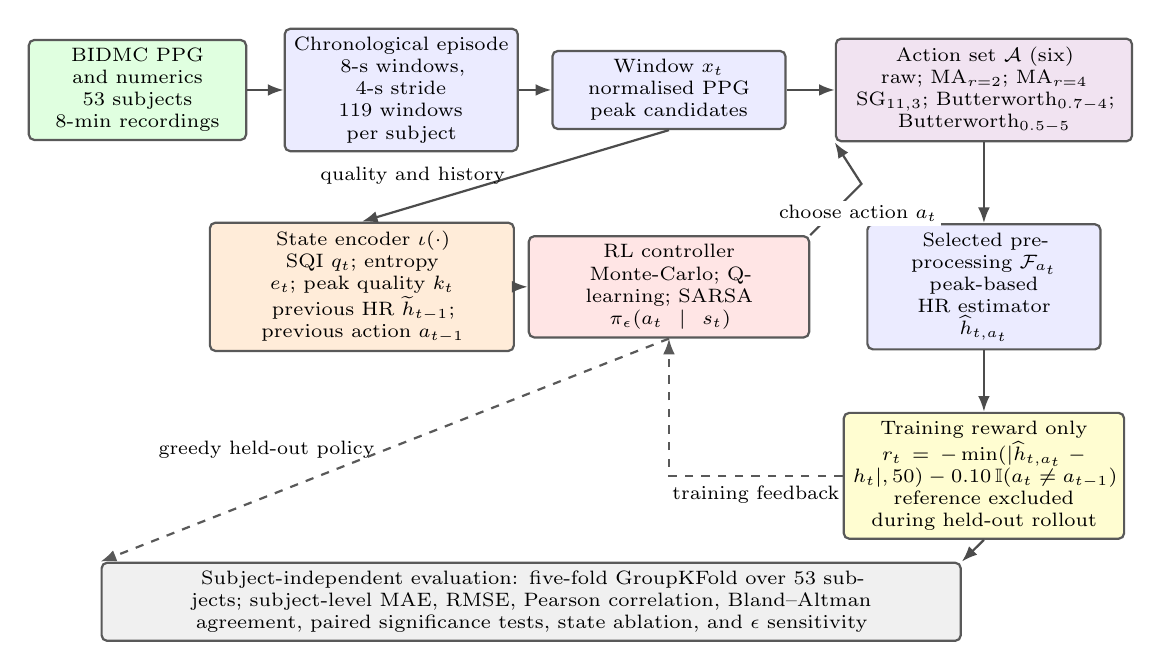
\begin{tikzpicture}[
  >=Latex,
  node distance=5mm and 7mm,
  fwbox/.style={draw=black!65, thick, rounded corners=2pt, align=center,
                inner sep=3pt, minimum height=9mm, font=\scriptsize},
  data/.style={fwbox, fill=green!12, text width=2.55cm},
  process/.style={fwbox, fill=blue!8, text width=2.75cm},
  statebox/.style={fwbox, fill=orange!15, text width=3.65cm},
  actionbox/.style={fwbox, fill=violet!11, text width=3.55cm},
  rlbox/.style={fwbox, fill=red!10, text width=3.35cm},
  rewardbox/.style={fwbox, fill=yellow!18, text width=3.35cm},
  evalbox/.style={fwbox, fill=gray!12, text width=10.7cm},
  fwarr/.style={-{Latex[length=2mm]}, thick, draw=black!70},
  fwfeedback/.style={-{Latex[length=2mm]}, thick, dashed, draw=black!65}
]
  \node[data] (data) at (-5.2,2.35)
    {BIDMC PPG and numerics\\53 subjects\\8-min recordings};
  \node[process] (episode) at (-1.85,2.35)
    {Chronological episode\\8-s windows, 4-s stride\\119 windows per subject};
  \node[process] (window) at (1.55,2.35)
    {Window $x_t$\\normalised PPG\\peak candidates};
  \node[actionbox] (filter) at (5.55,2.35)
    {Action set $\mathcal{A}$ (six)\\raw; MA$_{r=2}$; MA$_{r=4}$\\
     SG$_{11,3}$; Butterworth$_{0.7-4}$; Butterworth$_{0.5-5}$};

  \node[statebox] (state) at (-2.35,-0.15)
    {State encoder $\iota(\cdot)$\\
     SQI $q_t$; entropy $e_t$; peak quality $k_t$\\
     previous HR $\widetilde h_{t-1}$; previous action $a_{t-1}$};
  \node[rlbox] (agent) at (1.55,-0.15)
    {RL controller\\
     Monte-Carlo; Q-learning; SARSA\\
     $\pi_{\epsilon}(a_t\mid s_t)$};
  \node[process] (estimate) at (5.55,-0.15)
    {Selected preprocessing $\mathcal{F}_{a_t}$\\
     peak-based HR estimator\\
     $\widehat h_{t,a_t}$};
  \node[rewardbox] (reward) at (5.55,-2.55)
    {Training reward only\\
     $r_t=-\min(|\widehat h_{t,a_t}-h_t|,50)
     -0.10\,\mathbb{I}(a_t\ne a_{t-1})$\\
     reference excluded during held-out rollout};
  \node[evalbox] (evaluation) at (-0.2,-4.15)
    {Subject-independent evaluation: five-fold GroupKFold over 53 subjects;
     subject-level MAE, RMSE, Pearson correlation, Bland--Altman agreement,
     paired significance tests, state ablation, and $\epsilon$ sensitivity};

  \draw[fwarr] (data) -- (episode);
  \draw[fwarr] (episode) -- (window);
  \draw[fwarr] (window) -- (filter);
  \draw[fwarr] (window.south) -- node[left, font=\scriptsize]{quality and history}
    (state.north);
  \draw[fwarr] (state) -- (agent);
  \draw[fwarr] (agent.north east) -- ++(0.65,0.65) -- (filter.south west);
  \node[font=\scriptsize, fill=white, inner sep=1.5pt] at (3.95,0.78)
    {choose action $a_t$};
  \draw[fwarr] (filter.south) -- (estimate.north);
  \draw[fwarr] (estimate.south) -- (reward.north);
  \draw[fwfeedback] (reward.west) -| node[pos=0.25, below, font=\scriptsize]
    {training feedback} (agent.south);
  \draw[fwarr] (reward.south) -- (evaluation.north east);
  \draw[fwfeedback] (agent.south) -- node[left, font=\scriptsize]
    {greedy held-out policy} (evaluation.north west);
\end{tikzpicture}%
}
\caption{Framework for reinforcement learning-based adaptive filter selection
for PPG-derived heart-rate estimation. Consecutive windows form chronological
subject episodes; label-free state features drive selection among six
filter--parameter actions. The reference heart rate is used only to generate
training rewards and is not available to the held-out policy.}
\label{fig:framework}
\end{figure}

\subsection{Sequential RL formulation}

For an action $a_t$, the immediate reward is the clipped negative absolute error with a switching penalty:
\begin{equation}
 r_t=-\min\left(|\widehat h_{t,a_t}-h_t|,50\right)-0.10\,\mathbb{I}(a_t\ne a_{t-1}),
 \label{eq:reward}
\end{equation}
where $h_t$ is the window reference. The reward is evaluated only for training subjects; held-out rollout uses the learned table and observed state but never the held-out reference.

Every-visit Monte-Carlo learning accumulates discounted returns along each complete subject episode. For an episode of length $T$, the return from time $t$ is
\begin{equation}
 G_t=\sum_{k=t}^{T-1}\gamma^{k-t}r_k,
 \qquad
 Q_{\mathrm{MC}}(s,a)=\frac{1}{N(s,a)}\sum_{i:\,(s_i,a_i)=(s,a)}G_i,
 \label{eq:mc}
\end{equation}
where $N(s,a)$ is the every-visit count. Algorithm~\ref{alg:training}
summarizes the common training and held-out evaluation procedure.

Q-learning uses the off-policy update
\begin{equation}
 Q(s_t,a_t)\leftarrow Q(s_t,a_t)+\alpha_t\left[r_t+\gamma\max_aQ(s_{t+1},a)-Q(s_t,a_t)\right],
 \label{eq:q}
\end{equation}
where the terminal target omits the continuation term.

SARSA replaces the maximum with the value of the next action sampled from the same epsilon-greedy behaviour policy,
\begin{equation}
 Q(s_t,a_t)\leftarrow Q(s_t,a_t)+\alpha_t\left[r_t+\gamma Q(s_{t+1},a_{t+1})-Q(s_t,a_t)\right].
 \label{eq:sarsa}
\end{equation}
This on-policy target uses the action sampled from the same behaviour policy.

The contextual bandit uses the same state and action set but averages immediate rewards without a temporal bootstrap:
\begin{equation}
 Q_{\mathrm{CB}}(s_t,a_t)\leftarrow Q_{\mathrm{CB}}(s_t,a_t)+\frac{1}{N_t(s_t,a_t)}
 \left[r_t-Q_{\mathrm{CB}}(s_t,a_t)\right].
 \label{eq:bandit}
\end{equation}
For Q-learning and SARSA, $\alpha_t=0.10/\sqrt{n_t(s_t,a_t)}$ after the visit count is incremented and $\gamma=0.95$. The common exploration policy is
\begin{equation}
 \pi_{\epsilon}(a\mid s)=
 \frac{\epsilon}{|\mathcal{A}|}+
 \frac{1-\epsilon}{|\mathcal{G}(s)|}\mathbb{I}\{a\in\mathcal{G}(s)\},
 \qquad \mathcal{G}(s)=\arg\max_{a'\in\mathcal{A}}Q(s,a'),
 \qquad
 \epsilon_{r+1}=\max(0.05,0.97\epsilon_r).
 \label{eq:policy}
\end{equation}

\begin{algorithmblock}
\algtitle{Unified adaptive-filter training and evaluation}\label{alg:training}
\algrequire{Training subject episodes, action set $\mathcal{A}$, training-only
state encoder, update rule (Monte-Carlo, Q-learning, SARSA, or contextual bandit),
and an $\epsilon$-greedy schedule.}
\algensure{A learned action-value table and reference-blind predictions for every
held-out subject.}
\begin{algsteps}
\item Partition complete subjects into five grouped folds; fit state-bin edges
and initialization statistics on the training subjects only.
\item For each pass and chronological training episode, initialize the previous
estimate and action, encode $s_t$, select $a_t$, apply $\mathcal{F}_{a_t}$, and
compute $r_t$ from the training reference.
\item Update the table from complete returns (Monte-Carlo), the greedy next value
(Q-learning), the sampled next value (SARSA), or immediate reward only (bandit).
Decay $\epsilon$ after each pass.
\item Roll out the greedy policy on the held-out subjects without reference
access; retain chronological history and aggregate errors by subject.
\item Pool the 53 out-of-fold subject summaries and perform paired inference
with Holm correction.
\end{algsteps}
\end{algorithmblock}

All adaptive methods use epsilon-greedy action selection with uniform random exploration. The primary analysis uses three seeds (11, 22, and 33), 40 passes over the training episodes, an initial $\epsilon=1.0$, a minimum of 0.05, and multiplicative decay 0.97 after each pass. Ties among greedy actions are randomized. Fixed-filter baselines always select one action from Table~\ref{tab:actions}. The supervised baseline is a random-forest classifier trained on the state context \cite{kwon2024,gao2025,naeini2023}, with the training label equal to the action having the smallest observed training-window absolute error. This classifier is a strong, label-informed baseline, but it is not given held-out references.

The three temporal-learning algorithms share the same state encoder, reward, action set, episode order, and exploration schedule. Their executable procedures are placed immediately after their respective update equations so that each algorithm remains aligned with the surrounding explanation.

\begin{comment}
\begin{algorithmblock}
\algtitle{Every-visit Monte-Carlo filter selection}
\algrequire{Training episodes, state encoder $\iota(\cdot)$, action set $\mathcal{A}$, discount $\gamma$, and exploration schedule.}
\algensure{A state--action table $Q_{\mathrm{MC}}$ and a greedy held-out policy.}
\begin{enumerate}
\item Initialize $Q_{\mathrm{MC}}(s,a)=0$, $N(s,a)=0$, and the episode history.
\item For each chronological subject episode, initialize $\widetilde h_0$ and $a_0=-1$.
\item For $t=1,\ldots,T$, encode $s_t$, sample $a_t\sim\pi_\epsilon(\cdot\mid s_t)$, apply $\mathcal{F}_{a_t}$, estimate $\widehat h_{t,a_t}$, and store $(s_t,a_t,r_t)$.
\item Traverse the completed trajectory backward and set $G_T=0$ before computing
\begin{equation*}
 G_t=r_t+\gamma G_{t+1},\qquad
 N(s_t,a_t)\leftarrow N(s_t,a_t)+1,qquad
 Q_{\mathrm{MC}}(s_t,a_t)\leftarrow Q_{\mathrm{MC}}(s_t,a_t)+\frac{G_t-Q_{\mathrm{MC}}(s_t,a_t)}{N(s_t,a_t)}.
\end{equation*}
\item Decay $\epsilon$ after each training pass and return $\pi(s)=\arg\max_{a\in\mathcal{A}}Q_{\mathrm{MC}}(s,a)$.
\end{enumerate}
\end{algorithmblock}

\clearpage
\begin{algorithmblock}
\algtitle{Off-policy Q-learning filter selection}
\algrequire{Training episodes, encoded states, action set $\mathcal{A}$, $\gamma=0.95$, and $\alpha_t=0.10/\sqrt{N_t(s_t,a_t)}$.}
\algensure{An off-policy action-value table $Q$ and a greedy held-out policy.}
\begin{enumerate}
\item Initialize $Q(s,a)=0$ and visit counts $N(s,a)=0$.
\item For each training episode and time step $t$, encode $s_t$ and choose $a_t$ with $\epsilon$-greedy exploration.
\item Apply $\mathcal{F}_{a_t}$, obtain $r_t$ and $s_{t+1}$, and define the target
\begin{equation*}
y_t^{Q}=r_t+\gamma\mathbb{I}(t<T)\max_{a\in\mathcal{A}}Q(s_{t+1},a),qquad
Q(s_t,a_t)\leftarrow Q(s_t,a_t)+\alpha_t\left[y_t^{Q}-Q(s_t,a_t)\right].
\end{equation*}
\item At the terminal window, set $y_T^{Q}=r_T$; after all passes, select $\arg\max_{a\in\mathcal{A}}Q(s,a)$ during held-out rollout without using the reference heart rate.
\end{enumerate}
\end{algorithmblock}

\clearpage
\begin{algorithmblock}
\algtitle{On-policy SARSA filter selection}
\algrequire{Training episodes, encoded states, action set $\mathcal{A}$, $\gamma=0.95$, and the same $\epsilon$-greedy behaviour policy used by Q-learning.}
\algensure{An on-policy action-value table $Q_{\mathrm{SARSA}}$ and a greedy held-out policy.}
\begin{enumerate}
\item Initialize $Q_{\mathrm{SARSA}}(s,a)=0$ and visit counts $N(s,a)=0$.
\item At the first window of each episode, encode $s_t$ and select $a_t\sim\pi_\epsilon(\cdot\mid s_t)$.
\item Apply $\mathcal{F}_{a_t}$, observe $(r_t,s_{t+1})$, and select $a_{t+1}$ from the same behaviour policy.
\item Update with the sampled next action rather than the greedy action:
\begin{equation*}
y_t^{\mathrm{SARSA}}=r_t+\gamma\mathbb{I}(t<T)Q(s_{t+1},a_{t+1}),\qquad
Q_{\mathrm{SARSA}}(s_t,a_t)\leftarrow Q_{\mathrm{SARSA}}(s_t,a_t)+\alpha_t\left[y_t^{\mathrm{SARSA}}-Q_{\mathrm{SARSA}}(s_t,a_t)\right].
\end{equation*}
\item Set the terminal target to $y_T^{\mathrm{SARSA}}=r_T$; the final held-out rollout is greedy and preserves chronological previous-action and previous-heart-rate states.
\end{enumerate}
\end{algorithmblock}

\clearpage

\end{comment}

\subsection{Subject-independent evaluation}

Five-fold GroupKFold partitioning was performed using subject identity as the grouping variable. In each fold, approximately 42--43 subjects were used for training and 10--11 subjects were held out for testing. Every subject occurred in exactly one test fold; no overlapping windows from one subject crossed the train--test boundary. State bin edges, the initial reference rate, action-value tables, and the supervised classifier were fitted using the training subjects in each fold only.

Let $\mathcal{P}=\{1,\ldots,53\}$ denote the subjects and let $(\mathcal{T}_f,\mathcal{V}_f)$ be the training and test subject sets for fold $f$. The grouped design satisfies
\begin{equation}
 \mathcal{T}_f\cap\mathcal{V}_f=\varnothing,\qquad
 \mathcal{V}_f\cap\mathcal{V}_{f'}=\varnothing\ (f\ne f'),\qquad
 \bigcup_{f=1}^{5}\mathcal{V}_f=\mathcal{P},
 \label{eq:groupsplit}
\end{equation}
and all learned quantities in fold $f$ are functions of $\mathcal{T}_f$ only. This is the formal separation that prevents the correlated windows of one subject from appearing on both sides of a split.

The primary inference unit is the subject. For every method and subject, predictions from that subject's held-out windows were aggregated into subject-level MAE, RMSE, and Pearson correlation. The reported means and standard deviations therefore describe the 53 subject-level observations, not the much larger number of correlated windows. Bootstrap confidence intervals used 2000 resamples of subjects. Q-learning was the prespecified reference policy for paired comparisons. Two-sided paired $t$ tests and Wilcoxon signed-rank tests compared Q-learning with every other method, and Holm correction was applied to the Wilcoxon family at $\alpha=0.05$. Fold-level tests are reported only as exploratory because there are five folds.

\subsection{Evaluation metrics and agreement analysis}

For $N$ finite predictions, the principal error metrics are
\begin{equation}
 \operatorname{MAE}=\frac{1}{N}\sum_{i=1}^{N}|\widehat h_i-h_i|,
 \qquad
 \operatorname{RMSE}=\sqrt{\frac{1}{N}\sum_{i=1}^{N}(\widehat h_i-h_i)^2},
 \label{eq:metrics}
\end{equation}
and Pearson correlation is calculated between predicted and reference rates as a complementary association measure. For Bland--Altman analysis, $d_i=\widehat h_i-h_i$ and $m_i=(\widehat h_i+h_i)/2$; the bias and 95\% limits of agreement are
\begin{equation}
 \bar d=\frac{1}{N}\sum_{i=1}^{N}d_i,\qquad
 s_d=\sqrt{\frac{1}{N-1}\sum_{i=1}^{N}(d_i-\bar d)^2},\qquad
 \operatorname{LoA}_{\pm}=\bar d\pm1.96s_d.
 \label{eq:loa}
\end{equation}
Agreement summaries are descriptive because each subject contributes multiple overlapping windows. Metrics are first computed within each held-out subject and then averaged with equal subject weight, $\overline M_m=53^{-1}\sum_{p=1}^{53}M_{p,m}$. Paired differences $D_{p,m}=\operatorname{MAE}_{p,m}-\operatorname{MAE}_{p,Q}$ preserve the subject as the independent unit.

\begin{table}[h!]
\caption{Dataset, episode, and evaluation configuration.}
\label{tab:protocol}
\begin{center}
\small
\begin{tabular}{p{0.39\linewidth}p{0.48\linewidth}}
\toprule
Item & Setting \\
\midrule
Dataset & BIDMC PPG and Respiration Dataset v1.0.0 \\
Subjects and duration & 53 recordings; 8 min each \\
Sampling frequency & 125 Hz PPG; 1 Hz numerics \\
Window and stride & 8 s and 4 s \\
Windows & 119 per subject; 6307 total \\
Episode definition & Chronologically ordered windows within subject \\
Cross-validation & Five-fold subject-grouped cross-validation \\
Primary inference unit & Subject; $N=53$ \\
Agent seeds & 11, 22, 33 \\
Primary training passes & 40 episode passes \\
Primary exploration & $\epsilon_0=1.0$, $\epsilon_{\min}=0.05$, decay 0.97 \\
Bootstrap & 2000 subject resamples \\
\bottomrule
\end{tabular}
\end{center}
\vs{-4mm}
\end{table}

\section{Results}

\subsection{Protocol audit}

The completed run retained all 53 BIDMC subjects and generated 6307 consecutive windows. Every subject contributed 119 windows, spanning 0--479.99 s. The grouped split therefore held out complete subjects rather than randomly distributing highly overlapping windows. All six action specifications were evaluated in every fold, and the adaptive policies were trained on the same training subjects and tested on the same held-out subjects. The exported configuration, subject audit, window-level predictions, fold summaries, ablation data, and epsilon-sensitivity data are included with the analysis package.

\subsection{Primary subject-level comparison}

Table~\ref{tab:primary} reports subject-level means and standard deviations across all 53 subjects. Q-learning achieved MAE $3.840\pm8.965$ BPM, RMSE $5.198\pm9.329$ BPM, and correlation 0.274. The best fixed configuration by mean MAE was the third-order 0.7--4 Hz Butterworth filter, with MAE $3.819\pm8.956$ BPM and RMSE $5.021\pm9.335$ BPM. The difference in mean MAE between this fixed filter and Q-learning was 0.021 BPM, which is negligible relative to the between-subject standard deviation. The fixed 0.5--5 Hz fourth-order Butterworth filter was also competitive.

The adaptive methods did not form a uniformly ordered family. Q-learning had the lowest MAE among the learning policies, while the supervised action classifier had the highest mean correlation (0.281). Monte-Carlo and SARSA were close to the contextual bandit and Q-learning, indicating that the current state/action representation produces only modest separation among temporal credit-assignment strategies. The raw and smoothing baselines were similarly close, which shows that the task is not solved by a large global advantage for one preprocessing family.

\begin{table}[h!]
\caption{Primary subject-level performance across the 53 held-out subjects.}
\label{tab:primary}
\begin{center}
\small
\begin{tabular}{p{0.44\linewidth}ccc}
\toprule
Method & MAE (BPM) & RMSE (BPM) & Correlation \\
\midrule
Fixed: Butterworth 0.7--4 Hz, order 3 & 3.819 $\pm$ 8.956 & 5.021 $\pm$ 9.335 & 0.273 \\
Fixed: Butterworth 0.5--5 Hz, order 4 & 3.838 $\pm$ 8.963 & 5.168 $\pm$ 9.341 & 0.269 \\
Q-learning & 3.840 $\pm$ 8.965 & 5.198 $\pm$ 9.329 & 0.274 \\
Fixed: Savitzky--Golay & 3.854 $\pm$ 8.916 & 5.341 $\pm$ 9.307 & 0.267 \\
SARSA & 3.861 $\pm$ 8.969 & 5.272 $\pm$ 9.346 & 0.273 \\
Contextual bandit & 3.863 $\pm$ 8.993 & 5.248 $\pm$ 9.357 & 0.272 \\
Supervised action classifier & 3.863 $\pm$ 9.027 & 5.230 $\pm$ 9.379 & 0.281 \\
Fixed: raw & 3.878 $\pm$ 9.050 & 5.291 $\pm$ 9.376 & 0.276 \\
Monte-Carlo & 3.874 $\pm$ 8.971 & 5.292 $\pm$ 9.364 & 0.275 \\
Fixed: moving average 11 & 3.885 $\pm$ 8.925 & 5.401 $\pm$ 9.345 & 0.269 \\
Fixed: moving average 5 & 3.892 $\pm$ 9.027 & 5.303 $\pm$ 9.405 & 0.275 \\
\bottomrule
\end{tabular}
\end{center}
\vs{-4mm}
\end{table}

Bootstrap 95\% confidence intervals were $[1.856,6.490]$ BPM for the
best fixed filter's MAE and $[1.856,6.465]$ BPM for Q-learning. Window-level
failure rates were below 0.1\% for every adaptive method. Figure~\ref{fig:metrics}
reports confidence intervals for all principal metrics.

\subsection{Agreement and significance}

The subject-level Bland--Altman bias for Q-learning was $-2.347$ BPM, with the mean subject-level lower and upper limits of agreement at $-9.336$ and $4.641$ BPM, respectively. The corresponding bias for the best fixed Butterworth filter was $-2.413$ BPM, with limits $-9.356$ and $4.530$ BPM. These summaries indicate a small negative bias and broad subject-to-subject variability. The negative bias is not evidence that the adaptive policy is clinically interchangeable with a reference monitor; it describes the direction of error in this dataset and should be inspected together with the agreement plot.

Table~\ref{tab:significance} summarizes the primary paired tests. The unadjusted Wilcoxon comparison between Q-learning and the contextual bandit was $p=0.0587$, and the comparison with the best fixed Butterworth filter was $p=0.0804$. After Holm correction across the ten prespecified comparisons, the adjusted values were at least 0.5875. Consequently, the study does not demonstrate a statistically significant advantage of Q-learning over any comparator. This conclusion is consistent with the small numerical differences in Table~\ref{tab:primary}.

\begin{table}[h!]
\caption{Primary significance and Bland--Altman results for the main adaptive policies and the best fixed filter.}
\label{tab:significance}
\begin{center}
\small
\begin{tabular}{p{0.43\linewidth}ccc}
\toprule
Comparison or method & Wilcoxon $p$ & Holm $p$ & Bias (BPM) \\
\midrule
Q-learning vs contextual bandit & 0.0587 & 0.5875 & -- \\
Q-learning vs fixed Butterworth 0.7--4 Hz & 0.0804 & 0.6701 & -- \\
Q-learning vs SARSA & 0.1062 & 0.6701 & -- \\
Q-learning vs Monte-Carlo & 0.0900 & 0.6701 & -- \\
Q-learning & -- & -- & $-2.347$ \\
Fixed Butterworth 0.7--4 Hz & -- & -- & $-2.413$ \\
\bottomrule
\end{tabular}
\end{center}
\vs{-4mm}
\end{table}

\begin{figure}[h!]
\begin{center}
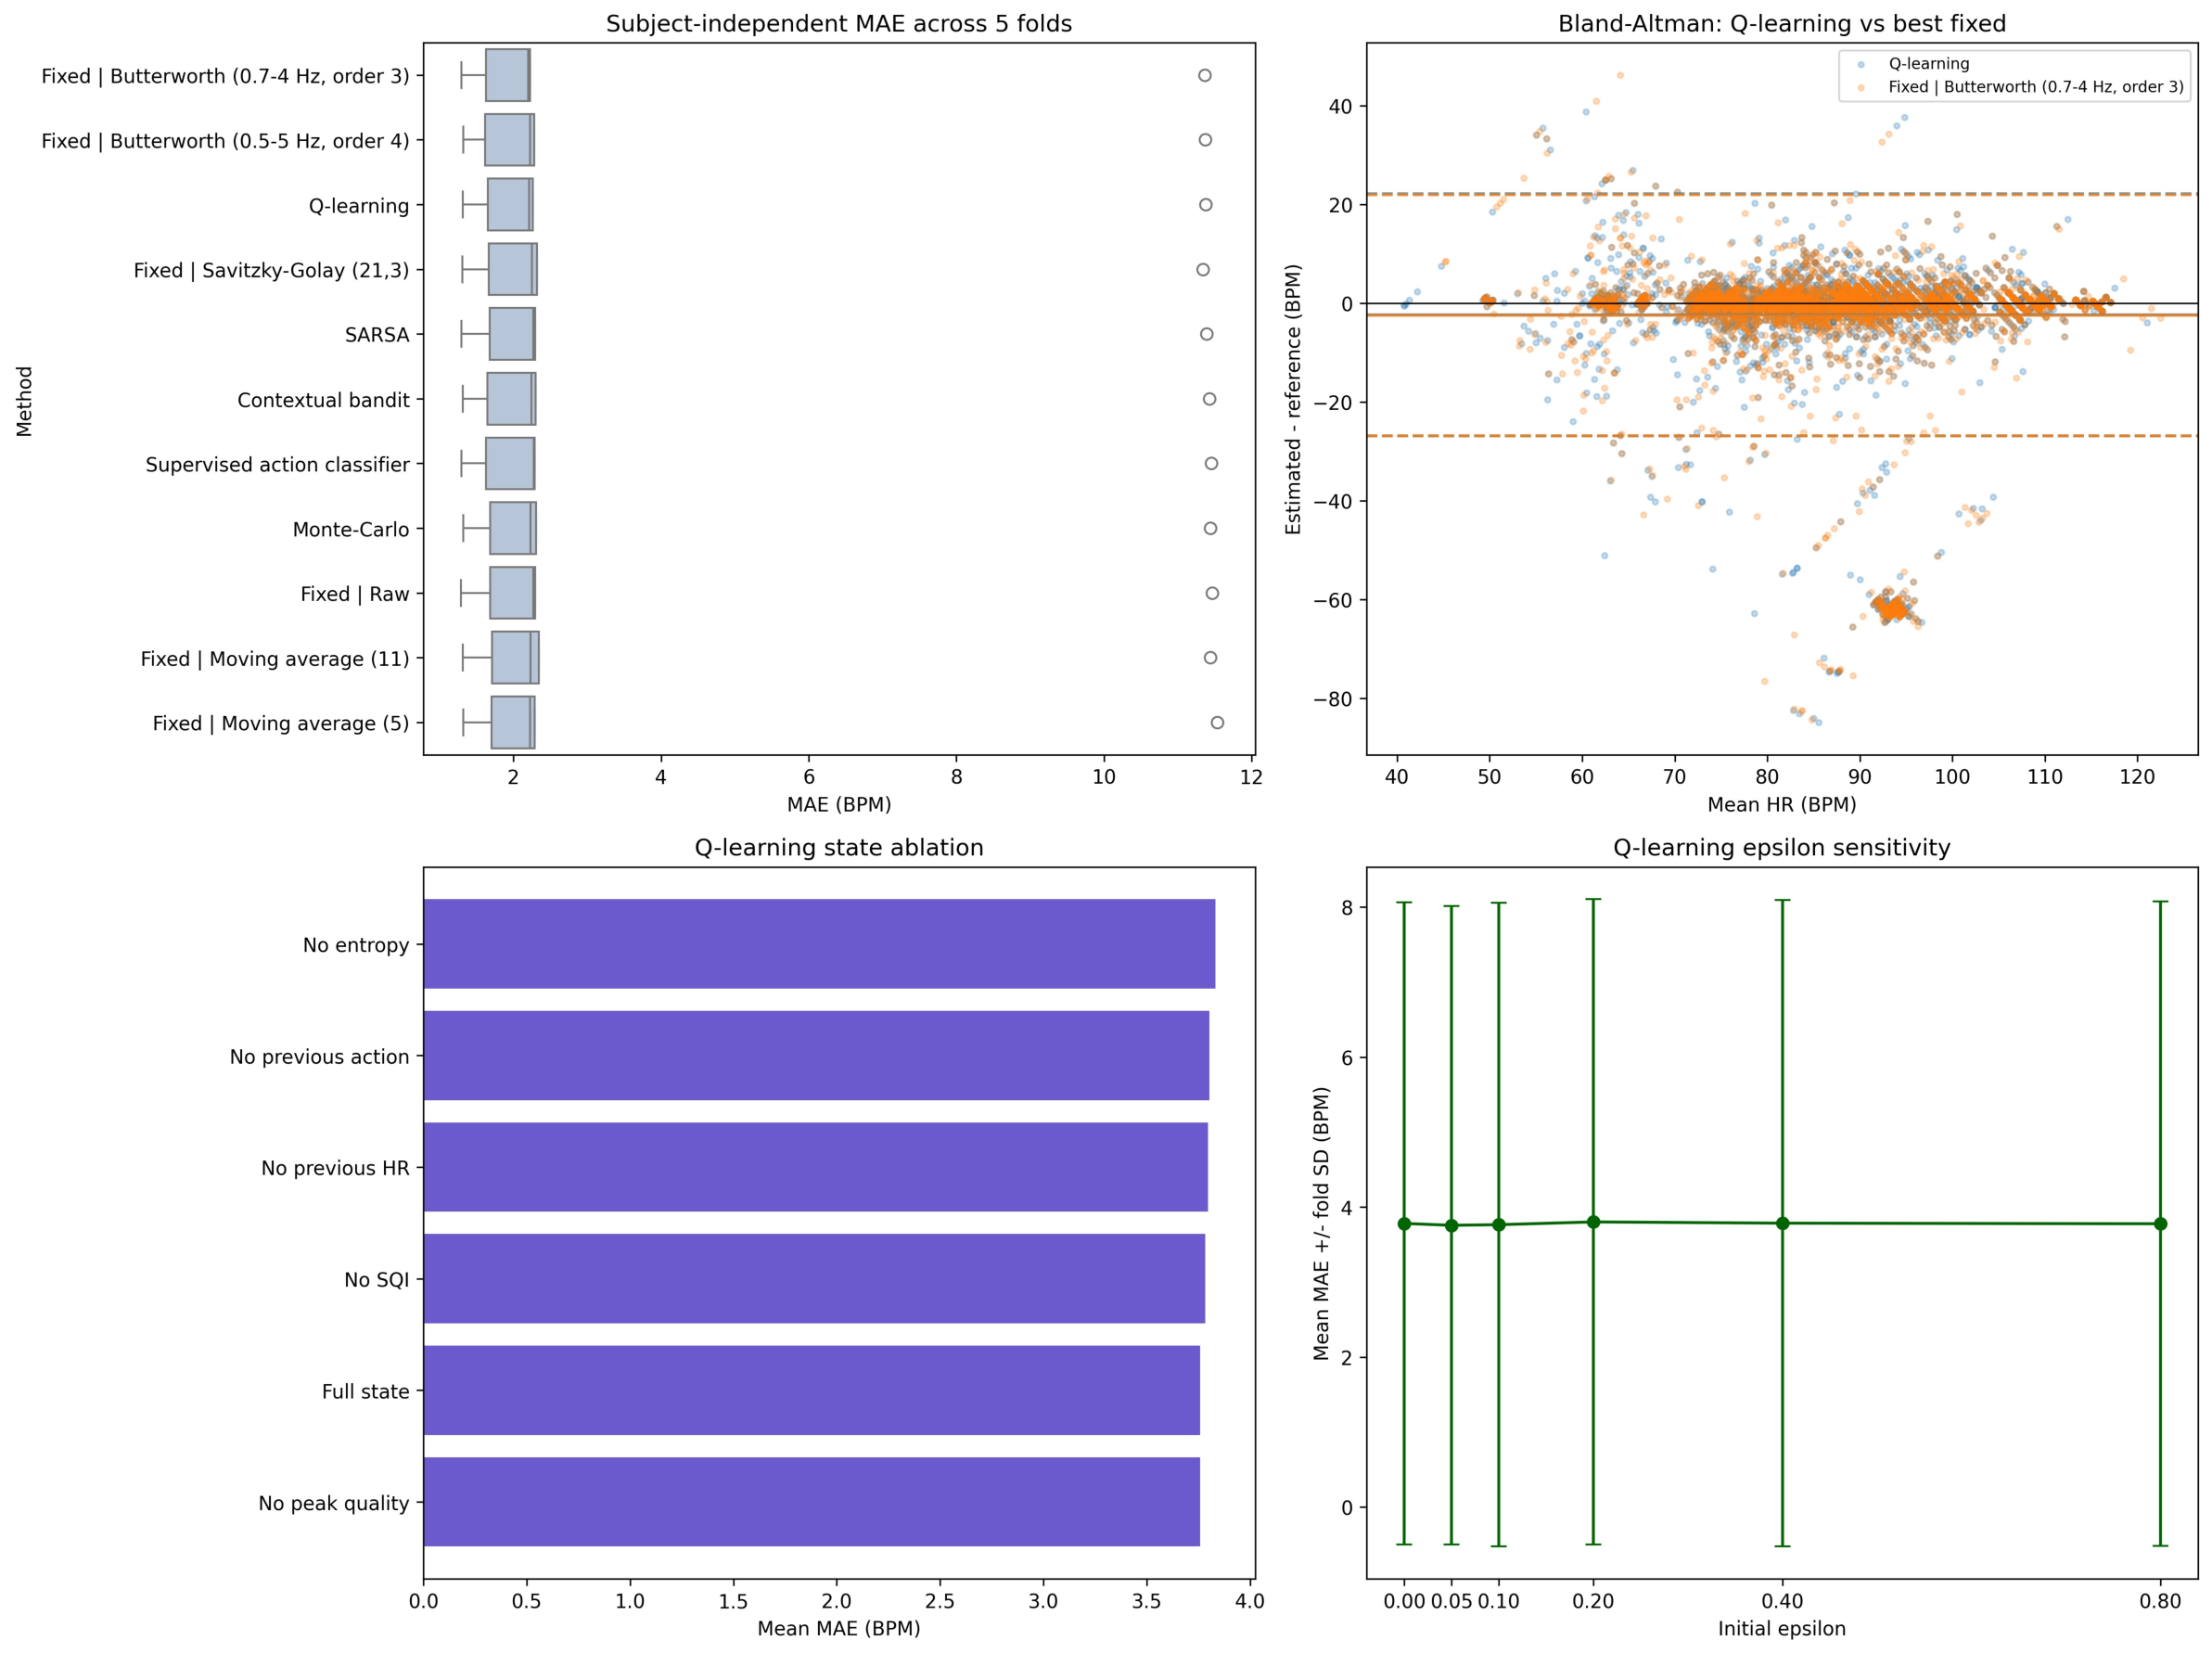
\includegraphics[width=16.0cm]{overview.pdf}
\caption{Overview of the completed subject-independent experiment. The panels show fold-level MAE distributions, Bland--Altman differences for Q-learning and the best fixed filter, state ablation, and initial-epsilon sensitivity.}
\label{fig:overview}
\end{center}
\vs{-4mm}
\end{figure}

\begin{figure}[h!]
\begin{center}
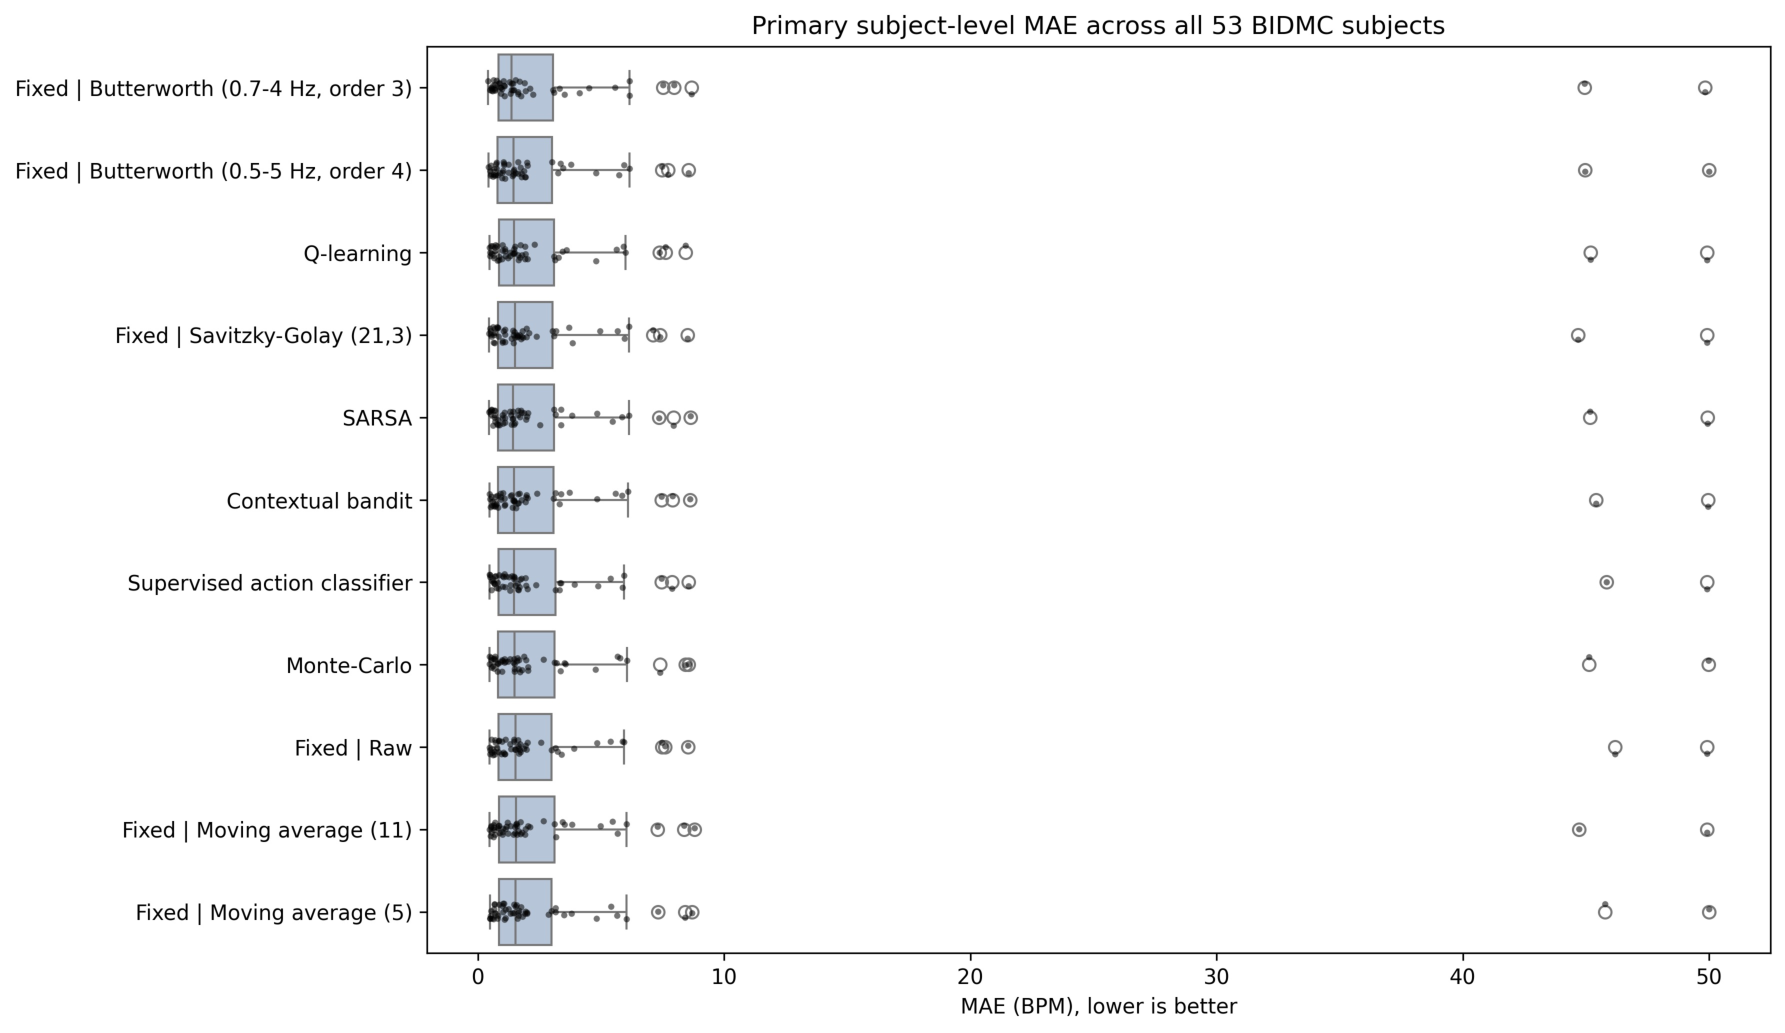
\includegraphics[width=15.5cm]{subject_level_mae.pdf}
\caption{Subject-level MAE for all 11 evaluated methods. Each point is one of the 53 subjects; the horizontal line denotes the method mean. The plot makes the between-subject heterogeneity visible rather than presenting only a pooled window estimate.}
\label{fig:subjectmae}
\end{center}
\vs{-4mm}
\end{figure}

\begin{figure}[h!]
\begin{center}
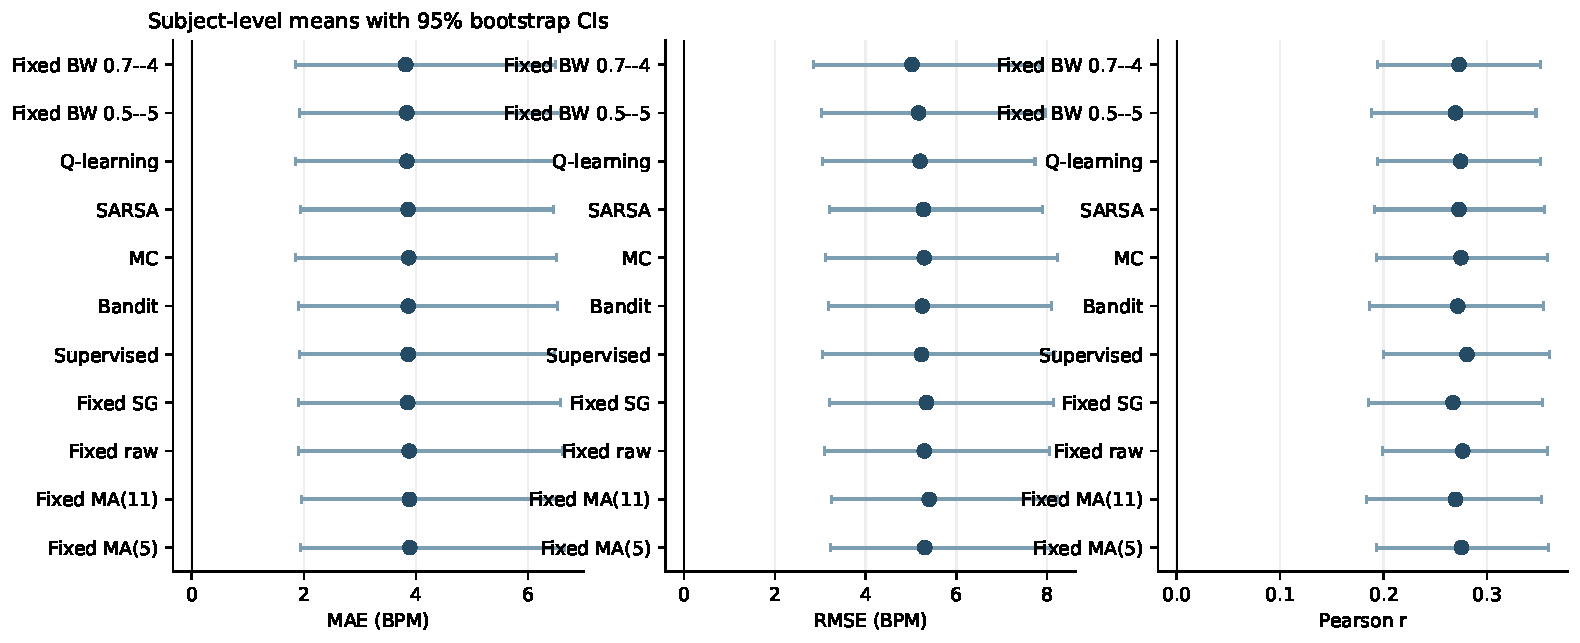
\includegraphics[width=15.5cm]{metric_comparison.pdf}
\caption{Subject-level MAE, RMSE, and Pearson correlation with bootstrap 95\% confidence intervals. MAE and RMSE are in BPM; correlation is dimensionless.}
\label{fig:metrics}
\end{center}
\vs{-4mm}
\end{figure}

\subsection{State ablation}

\begin{table}[h!]
\caption{Exploratory state-ablation and initial-exploration sensitivity across
five held-out folds. Values are mean $\pm$ fold-level standard deviation where
available.}
\label{tab:ablation}
\begin{center}
\small
\begin{tabular}{p{0.34\linewidth}ccc}
\toprule
Configuration & MAE (BPM) & RMSE (BPM) & Correlation \\
\midrule
\multicolumn{4}{l}{\textit{Panel A: state ablation}}\\
Full state & 3.758 $\pm$ 4.289 & 7.654 $\pm$ 7.984 & 0.767 \\
No SQI & 3.783 $\pm$ 4.320 & 7.690 $\pm$ 7.967 & 0.768 \\
No entropy & 3.833 $\pm$ 4.340 & 7.790 $\pm$ 7.960 & 0.761 \\
No peak quality & 3.757 $\pm$ 4.291 & 7.579 $\pm$ 7.977 & 0.769 \\
No previous HR & 3.795 $\pm$ 4.281 & 7.710 $\pm$ 7.915 & 0.766 \\
No previous action & 3.803 $\pm$ 4.307 & 7.800 $\pm$ 7.912 & 0.763 \\
\midrule
\multicolumn{4}{l}{\textit{Panel B: initial exploration $\epsilon_0$}}\\
$\epsilon_0=0.00$ & 3.782 $\pm$ 4.283 & 7.747 & 0.764 \\
$\epsilon_0=0.05$ & 3.757 $\pm$ 4.259 & 7.650 & 0.764 \\
$\epsilon_0=0.10$ & 3.765 $\pm$ 4.292 & 7.649 & 0.768 \\
$\epsilon_0=0.20$ & 3.802 $\pm$ 4.304 & 7.771 & 0.766 \\
$\epsilon_0=0.40$ & 3.785 $\pm$ 4.308 & 7.693 & 0.765 \\
$\epsilon_0=0.80$ & 3.778 $\pm$ 4.297 & 7.682 & 0.765 \\
\bottomrule
\end{tabular}
\end{center}
\vs{-4mm}
\end{table}

The state ablation used Q-learning with 25 passes per fold and is exploratory rather than a replacement for the primary 40-pass subject-level comparison. Removing entropy, previous action, or previous heart rate increased mean MAE from 3.758~BPM to 3.833, 3.803, and 3.795~BPM, respectively. Removing peak quality changed MAE by only $-0.001$~BPM. The pattern supports further evaluation of entropy and history but does not establish that every component is necessary.

\subsection{Exploration sensitivity}

Initial $\epsilon$ values of 0, 0.05, 0.10, 0.20, 0.40, and 0.80 were tested with 25 passes per fold. Their equal-fold mean MAEs are reported in Table~\ref{tab:ablation}. The lowest observed value occurred at $\epsilon_0=0.05$, but the fold standard deviations were 4.26--4.31~BPM and no multiple-seed inference was planned; the ranking is therefore descriptive.

\section{Discussion}

\subsection{Principal findings}

The central result is negative in the most useful scientific sense: adaptive RL filter selection was feasible and reproducible, but the current policy did not outperform a well-chosen fixed filter on the complete 53-subject BIDMC evaluation. Q-learning was numerically competitive and had the best MAE among the adaptive learning policies, but the third-order 0.7--4 Hz Butterworth baseline was slightly better. The difference was not significant, and all adjusted paired tests were non-significant. A paper that reported only the best adaptive number without this fixed-filter comparison would give an incomplete account of the evidence.

Several aspects of the result are informative. First, the contextual bandit was close to Q-learning, indicating that the value of temporal bootstrapping is modest under the present window-level reward and compact state representation. Second, SARSA and Monte-Carlo learning did not establish a consistent advantage over Q-learning. Third, the supervised classifier was not uniformly superior despite being trained to imitate the lowest-error action on training windows. These observations suggest that action predictability from local quality features is only part of the problem; the remaining error may be dominated by limitations of the peak estimator, the reference channel, or subject-specific morphology that is not represented by the five state variables.

\subsection{Signal-processing interpretation}

The best fixed action was a conventional band-pass filter with a cardiac passband. This is plausible: the BIDMC recordings were acquired in a controlled clinical setting, so the signal distribution may be sufficiently stable for a single filter to perform well. Adaptive switching introduces two potential costs. It can select a locally reasonable filter whose peak detector fails on a difficult morphology, and it can create temporal discontinuity through the previous-action penalty or through changes in waveform shape between adjacent windows. The ablation result for previous action is consistent with this trade-off: removing it increased error in the exploratory analysis, suggesting that action history contains useful persistence information, but it does not establish that the switching penalty itself is optimal.

The use of zero-phase filtering is appropriate for retrospective benchmarking because it avoids phase displacement, but it is not causal. A real-time deployment would need causal IIR filtering, a causal smoother, or an explicitly compensated delay. The paper therefore evaluates adaptive filter selection as an offline methodological benchmark, not as a ready-to-deploy real-time implementation. This distinction should be retained in any clinical or wearable-sensor claim.

\subsection{Statistical interpretation and limitations}

The large subject-level standard deviations show that performance is heterogeneous. Subjects with unusual pulse morphology or large reference variation can dominate means, which is why the analysis reports subject-level confidence intervals and paired tests rather than treating thousands of overlapping windows as independent replicates. The confidence intervals are also wide, so a larger independent cohort may be needed to detect small differences of the magnitude observed here.

The study has five important limitations. First, the dataset contains 53 recordings, all from the same public source and each only eight minutes long; external validation is required before generalization. Second, the monitor PULSE channel is used as the reference, so the experiment measures agreement with a monitor-derived pulse-rate channel rather than an independently adjudicated electrocardiographic reference. Third, the peak detector and the quality features are hand-designed, and errors in those components can mask a benefit from the policy. Fourth, the action space is intentionally small: it contains six fixed parameterizations rather than a continuous filter-design space. Fifth, the RL reward uses a clipped absolute error and a fixed switching penalty; alternative rewards, continuous actions, causal filters, and deep policies such as deep Q-networks or recurrent actor--critic methods remain untested.

The current results also motivate a careful interpretation of deep RL extensions. A deep Q-network or a recurrent policy could represent richer histories, but it would introduce additional hyperparameters and a greater risk of fitting subject-specific patterns. Such models should be evaluated under the same grouped splits, with repeated subject-level seeds, calibration of action probabilities, and a predeclared computational budget. Adding model capacity without strengthening the evaluation would not address the main limitation revealed here.

\section{Conclusion}

This study presented a complete, subject-independent benchmark for reinforcement learning-based adaptive filter selection in PPG-derived heart-rate estimation. All 53 BIDMC subjects were used, and each recording was represented as a chronological 119-window episode. The state included signal-quality index, entropy, peak quality, previous heart rate, and previous action; actions explicitly encoded filter families and parameters. Monte-Carlo, Q-learning, SARSA, contextual bandit, fixed-filter, and supervised baselines were evaluated with MAE, RMSE, correlation, Bland--Altman analysis, paired significance tests, state ablation, and epsilon sensitivity.

Q-learning was competitive but did not significantly improve on the best fixed Butterworth filter. The appropriate conclusion is therefore not that RL has failed, but that the present adaptive formulation has not yet earned a superiority claim. The released notebook and exported tables make the negative and positive findings auditable. Future work should add independent cohorts, causal filtering, repeated seeds, a stronger reference standard, and carefully budgeted continuous or deep policies. Until those tests are completed, the fixed-filter result is an important baseline and adaptive selection should be presented as a promising framework rather than a clinically validated replacement.

\section*{Acknowledgment and/or disclaimers}

The author acknowledges the BIDMC dataset contributors and PhysioNet.

\section*{Declaration of generative AI and AI-assisted technologies}

During preparation of this manuscript, the author used OpenAI Codex for
language editing, \LaTeX{} formatting, and submission-guideline checks. The
tool was not used to generate or alter research data, execute the reported
statistical analysis, or make scientific decisions. The author reviewed and
edited all AI-assisted output and assumes full responsibility for the content
of the manuscript.


\section*{Data availability statement}

The BIDMC PPG and Respiration Dataset v1.0.0 is publicly available from PhysioNet at \texttt{https://doi.org/10.13026/C2208R}. The analysis notebook and exported result files are supplied as supplementary material.

\section*{Funding}

This research received no external funding.

\section*{Conflict of interest}

The author declares no conflict of interest.

\section*{Informed consent}

Not applicable. This study is a secondary analysis of a de-identified public dataset and involved no new human-participant procedures.

\begin{thebibliography}{99}

\bibitem{charlton2023}
Charlton PH, Allen J, Bail\'on R, Baker S, Behar JA et al. The 2023 wearable photoplethysmography roadmap. Physiological Measurement 2023; 44 (11): 111001. https://doi.org/10.1088/1361-6579/acead2

\bibitem{kyriacou2026}
Kyriacou PA. Standardizing photoplethysmography (PPG) for clinical-grade wearable sensing. Biomedical Signal Processing and Control 2026; 127: 110991. https://doi.org/10.1016/j.bspc.2026.110991

\bibitem{wearablefusion2023}
Wen H, Gao B, Yang D, Zhang Y, Huang L, Woo WL. Wearable integrated online fusion learning filter for heart PPG sensing tracking. IEEE Sensors Journal 2023; 23: 14938--14949. https://doi.org/10.1109/JSEN.2023.3277719

\bibitem{wrist2023}
Hasan K, Chowdhury MH, Pathan NS, Hossain QD. Heart rate estimation from wrist PPG signal during intense physical exercise. SN Computer Science 2023; 4. https://doi.org/10.1007/s42979-023-02173-6

\bibitem{hao2024}
Hao Z, Wang J, Zhang G, Gao L, Zhang X et al. PPG heart rate extraction algorithm based on the motion artifact intensity classification and removal framework. Biomedical Signal Processing and Control 2024; 94: 106287. https://doi.org/10.1016/j.bspc.2024.106287

\bibitem{sicbaldi2025}
Sicbaldi M, Palmerini L, Moscato S, di Florio P, Silvani A, Chiari L. Benchmarking of open-source algorithms for heart rate estimation from motion-corrupted photoplethysmography. Computers in Biology and Medicine 2025; 196: 110808. https://doi.org/10.1016/j.compbiomed.2025.110808

\bibitem{naeini2023}
Naeini EK, Sarhaddi F, Azimi I, Liljeberg P, Dutt ND, Rahmani AM. A deep learning-based PPG quality assessment approach for heart rate and heart rate variability. ACM Transactions on Computing for Healthcare 2023; 4 (4): Article 24. https://doi.org/10.1145/3616019

\bibitem{schmith2023}
Schmith J, Kelsch C, Cappelozza Cunha B, Prade LR, Martins EA et al. Photoplethysmography signal quality assessment using attractor reconstruction analysis. Biomedical Signal Processing and Control 2023; 86: 105142. https://doi.org/10.1016/j.bspc.2023.105142

\bibitem{sarkar2024}
Sarkar S, Ghosh A, Alam S, Datta S, Dutta A et al. Schr\"odinger spectrum and slim CNN architecture-based signal quality estimation for photoplethysmogram signals. Biomedical Signal Processing and Control 2024; 94: 106240. https://doi.org/10.1016/j.bspc.2024.106240

\bibitem{determinants2025}
Charlton PH, Marozas V, Mej\'ia-Mej\'ia E, Kyriacou PA, Mant J. Determinants of photoplethysmography signal quality at the wrist. PLOS Digital Health 2025; 4: e0000585. https://doi.org/10.1371/journal.pdig.0000585

\bibitem{sutton2018}
Sutton RS, Barto AG. Reinforcement Learning: An Introduction. 2nd ed. Cambridge, MA, USA: MIT Press; 2018.

\bibitem{beh2024}
Beh W-K, Yang Y-C, Wu A-Y. Quality-aware signal processing mechanism of PPG signal for long-term heart rate monitoring. Sensors 2024; 24 (12): 3901. https://doi.org/10.3390/s24123901

\bibitem{guo2026}
Guo J, Chen S, Lan T, Li R, Wang L et al. Research on heart rate estimation algorithm based on dynamic PPG. Frontiers in Signal Processing 2026; 6: 1724468. https://doi.org/10.3389/frsip.2026.1724468

\bibitem{pimentel2017}
Pimentel MAF, Johnson AEW, Charlton PH, Birrenkott D, Watkinson PJ et al. Towards a robust estimation of respiratory rate from pulse oximeters. IEEE Transactions on Biomedical Engineering 2017; 64 (8): 1914--1923. https://doi.org/10.1109/TBME.2016.2613124

\bibitem{kwon2024}
Kwon T, Yoon SW. Anomaly detection of motion artifact in photoplethysmography sensors using unsupervised learning. IEEE Sensors Journal 2024; 24: 23163--23172. https://doi.org/10.1109/JSEN.2024.3404558

\bibitem{gao2025}
Gao R, Miller CS, Lin BTW, Schwarz CW, Jones MLH. Signal quality assessment and reconstruction of PPG-derived signals for heart rate and variability estimation in in-vehicle applications: a comparative review and empirical validation. Sensors 2025; 25 (24): 7556. https://doi.org/10.3390/s25247556

\end{thebibliography}

\begin{comment}

\bibitem{naeini2023}
Naeini EK, Sarhaddi F, Azimi I, Liljeberg P, Dutt ND, Rahmani AM. A deep learning-based PPG quality assessment approach for heart rate and heart rate variability. ACM Transactions on Computing for Healthcare 2023; 4 (4): Article 24. https://doi.org/10.1145/3616019

\bibitem{charlton2023}
Charlton PH, Allen J, Bailón R, Baker S, Behar JA et al. The 2023 wearable photoplethysmography roadmap. Physiological Measurement 2023; 44 (11): 111001. https://doi.org/10.1088/1361-6579/acead2

\bibitem{slider2023}
McLean MK, Weaver RG, Lane A, Smith MT, Parker H, Stone B, McAninch J, Matolak DW, Burkart S, Chandrashekhar MVS, Armstrong B. A sliding scale signal quality metric of photoplethysmography applicable to measuring heart rate across clinical contexts with chest mounting as a case study. Sensors 2023; 23 (7): 3429. https://doi.org/10.3390/s23073429

\bibitem{interference2023}
Qi Y, Zhang A, Ma Y, Wang H, Li J. Interference source-based quality assessment method for postauricular photoplethysmography signals. Biomedical Signal Processing and Control 2023; 84: 104751. https://doi.org/10.1016/j.bspc.2023.104751

\bibitem{schmith2023}
Schmith J, Kelsch C, Cappelozza Cunha B, Prade LR, Martins EA, Keller AL, de Figueiredo RM. Photoplethysmography signal quality assessment using attractor reconstruction analysis. Biomedical Signal Processing and Control 2023; 86: 105142. https://doi.org/10.1016/j.bspc.2023.105142

\bibitem{wearablefusion2023}
Wen H, Gao B, Yang D, Zhang Y, Huang L, Woo WL. Wearable integrated online fusion learning filter for heart PPG sensing tracking. IEEE Sensors Journal 2023; 23: 14938--14949. https://doi.org/10.1109/JSEN.2023.3277719

\bibitem{wrist2023}
Hasan K, Chowdhury MH, Pathan NS, Hossain QD. Heart rate estimation from wrist PPG signal during intense physical exercise. SN Computer Science 2023; 4. https://doi.org/10.1007/s42979-023-02173-6

\bibitem{antimotion2023}
Duan Y, He C, Zhou M. Anti-motion imaging photoplethysmography via self-adaptive multi-ROI tracking and selection. Physiological Measurement 2023; 44: 115003. https://doi.org/10.1088/1361-6579/ad071f

\bibitem{grgb2023}
Haugg F, Elgendi M, Menon C. GRGB rPPG: an efficient low-complexity remote photoplethysmography-based algorithm for heart rate estimation. Bioengineering 2023; 10 (2): 243. https://doi.org/10.3390/bioengineering10020243

\bibitem{unet2023}
Yu S-N, Wang C-S, Chang Y-P. Heart rate estimation from remote photoplethysmography based on lightweight U-Net and attention modules. IEEE Access 2023; 11: 54058--54069. https://doi.org/10.1109/ACCESS.2023.3281898

\bibitem{remotereview2023}
Lee RJ, Sivakumar S, Lim KH. Review on remote heart rate measurements using photoplethysmography. Multimedia Tools and Applications 2024; 83: 44699--44728. https://doi.org/10.1007/s11042-023-16794-9

\bibitem{remotereview2024}
Xiao H, Liu T, Sun Y, Li Y, Zhao S, Avolio A. Remote photoplethysmography for heart rate measurement: a review. Biomedical Signal Processing and Control 2024; 88: 105608. https://doi.org/10.1016/j.bspc.2023.105608

\bibitem{beh2024}
Beh W-K, Yang Y-C, Wu A-Y. Quality-aware signal processing mechanism of PPG signal for long-term heart rate monitoring. Sensors 2024; 24 (12): 3901. https://doi.org/10.3390/s24123901

\bibitem{arguello2024}
Argüello-Prada EJ, Castillo García JF. Machine learning applied to reference signal-less detection of motion artifacts in photoplethysmographic signals: a review. Sensors 2024; 24 (22): 7193. https://doi.org/10.3390/s24227193

\bibitem{hao2024}
Hao Z, Wang J, Zhang G, Gao L, Zhang X, Liu J, Zhang X, Yang X, Lai Z. PPG heart rate extraction algorithm based on the motion artifact intensity classification and removal framework. Biomedical Signal Processing and Control 2024; 94: 106287. https://doi.org/10.1016/j.bspc.2024.106287

\bibitem{sarkar2024}
Sarkar S, Ghosh A, Alam S, Datta S, Dutta A, Choudhury A, Pal A. Schrödinger spectrum and slim CNN architecture-based signal quality estimation for photoplethysmogram signals. Biomedical Signal Processing and Control 2024; 94: 106240. https://doi.org/10.1016/j.bspc.2024.106240

\bibitem{kwon2024}
Kwon T, Yoon SW. Anomaly detection of motion artifact in photoplethysmography sensors using unsupervised learning. IEEE Sensors Journal 2024; 24: 23163--23172. https://doi.org/10.1109/JSEN.2024.3404558

\bibitem{dilernia2024}
Di Lernia D, Finotti G, Tsakiris M, Riva G, Naber M. Remote photoplethysmography in the wild: remote heart rate imaging via online webcams. Behavior Research Methods 2024; 56: 6904--6914. https://doi.org/10.3758/s13428-024-02398-0

\bibitem{pirzada2024}
Pirzada P, Wilde A, Harris-Birtill D. Remote photoplethysmography for heart rate and blood oxygenation measurement: a review. IEEE Sensors Journal 2024; 24: 23436--23453. https://doi.org/10.1109/JSEN.2024.3405414

\bibitem{shin2024}
Shin H. Signal completion using generative adversarial networks for enhanced photoplethysmography measurement accuracy. Computers in Biology and Medicine 2024; 180: 108952. https://doi.org/10.1016/j.compbiomed.2024.108952

\bibitem{wu2024}
Wu H. Multiscale entropy with electrocardiograph, electromyography, electroencephalography, and photoplethysmography signals in healthcare: a twelve-year systematic review. Biomedical Signal Processing and Control 2024; 93: 106124. https://doi.org/10.1016/j.bspc.2024.106124

\bibitem{gao2025}
Gao R, Miller CS, Lin BTW, Schwarz CW, Jones MLH. Signal quality assessment and reconstruction of PPG-derived signals for heart rate and variability estimation in in-vehicle applications: a comparative review and empirical validation. Sensors 2025; 25 (24): 7556. https://doi.org/10.3390/s25247556

\bibitem{wang2025}
Wang J, Hui H, Yang H, Xie P, Ji Z. A lightGBM-based method for the signal quality assessment of wrist photoplethysmography. Physical and Engineering Sciences in Medicine 2025; 48: 1715--1728. https://doi.org/10.1007/s13246-025-01616-z

\bibitem{sicbaldi2025}
Sicbaldi M, Palmerini L, Moscato S, di Florio P, Silvani A, Chiari L. Benchmarking of open-source algorithms for heart rate estimation from motion-corrupted photoplethysmography. Computers in Biology and Medicine 2025; 196: 110808. https://doi.org/10.1016/j.compbiomed.2025.110808

\bibitem{determinants2025}
Charlton PH, Marozas V, Mejía-Mejía E, Kyriacou PA, Mant J. Determinants of photoplethysmography signal quality at the wrist. PLOS Digital Health 2025; 4: e0000585. https://doi.org/10.1371/journal.pdig.0000585

\bibitem{bondarenko2025}
Bondarenko M, Menon C, Elgendi M. The role of face regions in remote photoplethysmography for contactless heart rate monitoring. npj Digital Medicine 2025; 8. https://doi.org/10.1038/s41746-025-01814-9

\bibitem{chen2025}
Chen C-C, Lin S-X, Jeong H. Low-complexity timing correction methods for heart rate estimation using remote photoplethysmography. Sensors 2025; 25 (2): 588. https://doi.org/10.3390/s25020588

\bibitem{gupta2025}
Gupta A, Devasahayam SR, Subudhi BN. Heart rate and HRV estimation using PPG based on Superlet transform and LSTM network. IEEE Transactions on Instrumentation and Measurement 2025; 74: 1--11. https://doi.org/10.1109/TIM.2025.3606047

\bibitem{guo2026}
Guo J, Chen S, Lan T, Li R, Wang L, Wu Y, Zhong J, Zhu W. Research on heart rate estimation algorithm based on dynamic PPG. Frontiers in Signal Processing 2026; 6: 1724468. https://doi.org/10.3389/frsip.2026.1724468

\bibitem{ricci2026}
Ricci F, Vivarelli C, Mattei E, Calcagnini G. Signal quality of reflective-mode photoplethysmograms across anatomical sites. Sensors 2026; 26 (10): 2986. https://doi.org/10.3390/s26102986

\bibitem{tian2026}
Tian Y, Li S, Zhu Y, Elgendi M, Lam EY. Adaptive physiology-informed correction for reliable remote photoplethysmography heart-rate monitoring. npj Digital Medicine 2026; 9. https://doi.org/10.1038/s41746-026-02386-y

\bibitem{kyriacou2026}
Kyriacou PA. Standardizing photoplethysmography (PPG) for clinical-grade wearable sensing. Biomedical Signal Processing and Control 2026; 127: 110991. https://doi.org/10.1016/j.bspc.2026.110991

\bibitem{xue2026}
Xue Q, Zhang Y, Wu H, Song Y. Transformer-based contrastive learning for remote photoplethysmography signal recovery amid landmark loss. Biomedical Signal Processing and Control 2026; 127: 111086. https://doi.org/10.1016/j.bspc.2026.111086

\bibitem{ppgsport2026}
Hu C, Pham HM, Zhang Y, Yan G, Ma X, Wu Y, Kandappu T, Misra A, Ma D. PPG-Sport: a dataset for reliable heart rate monitoring from wrist PPG under dynamic sports conditions. Proceedings of the ACM on Interactive, Mobile, Wearable and Ubiquitous Technologies 2026; 10: 1--28. https://doi.org/10.1145/3810216

\bibitem{deb2026}
Debnath U, Kim S. Advanced signal-processing framework for remote photoplethysmography-based heart rate measurement: integrating adaptive Kalman filtering with discrete wavelet transformation. PLOS ONE 2026; 21: e0340097. https://doi.org/10.1371/journal.pone.0340097

\bibitem{elgendi2026}
Elgendi M, Li S, Menon C, Lam EY, Al-Omari B, Borik S, Shelley KH, Alian A. Roadmap of remote photoplethysmography from heart rate measurement toward clinical translation. npj Digital Medicine 2026; 9. https://doi.org/10.1038/s41746-026-02715-1

\end{comment}

\end{document}
